\documentclass[11pt]{article}
\usepackage{latexsym}
\usepackage{amsmath}
\usepackage{amssymb}
\usepackage{amsthm}
\usepackage{epsfig}
\usepackage[tight]{subfigure}
\usepackage{xcolor}

\usepackage{amsmath}

\DeclareMathOperator*{\minimize}{min}
\DeclareMathOperator*{\maximize}{max}

\usepackage{algorithm}
 %on linux you may need to run sudo apt-get install texlive-full to install algorithm.sys
\usepackage{algorithmic}

\usepackage{verbatim}

\newcommand{\handout}[5]{
  \noindent
  \begin{center}
  \framebox{
    \vbox{
      \hbox to 5.78in { {#1} \hfill #2 }
      \vspace{4mm}
      \hbox to 5.78in { {\Large \hfill #5  \hfill} }
      \vspace{2mm}
      \hbox to 5.78in { {\em #3 \hfill #4} }
    }
  }
  \end{center}
  \vspace*{4mm}
}

\newcommand{\lecture}[5]{\handout{#1}{#2}{#3}{#4}{#5}}
\newcommand{\collision}[0]{\mathrm{collision}}
\newcommand{\nocollision}[0]{\overline{\collision}}

\newcommand*{\QED}{\hfill\ensuremath{\square}}

\newtheorem{theorem}{Theorem}
\newtheorem{corollary}[theorem]{Corollary}
\newtheorem{lemma}[theorem]{Lemma}
\newtheorem{observation}[theorem]{Observation}
\newtheorem{proposition}[theorem]{Proposition}
\newtheorem{definition}[theorem]{Definition}
\newtheorem{claim}[theorem]{Claim}
\newtheorem{fact}[theorem]{Fact}
\newtheorem{assumption}[theorem]{Assumption}
\newtheorem{note}[theorem]{Note}

% 1-inch margins, from fullpage.sty by H.Partl, Version 2, Dec. 15, 1988.
\topmargin 0pt
\advance \topmargin by -\headheight
\advance \topmargin by -\headsep
\textheight 8.9in
\oddsidemargin 0pt
\evensidemargin \oddsidemargin
\marginparwidth 0.5in
\textwidth 6.5in

\parindent 0in
\parskip 1.5ex
%\renewcommand{\baselinestretch}{1.25}

\begin{document}

\lecture{Statistical Techniques in Robotics (16-831, S21)}{Lecture \#25
  (Wednesday, May 5)}{Lecturer: Kris Kitani}{Scribes: Xuhua Huang, Xinjie Yao}{Passive Imitation Learning \& Interactive Imitation Learning}

\section{Review}
This is the final lecture of this semester. First of all, great thanks to \textbf{Kris Kitani} and \textbf{Xingyu Lin} for such a great learning experience! In the last lecture, we get started on a new topic called Imitation Learning (IL), which is a method aiming to learn and develop own skills by observing skills performed by others. As a high-level summary, we have:
\begin{table}[H]
\centering
\begin{tabular}{|c|c|c|c|}
\hline & Passive IL & Active IL & Interactive IL \\
\hline Demonstrations $\mathcal{D}$ & yes & yes & optional \\
\hline Environment $\mathcal{E}$ & no & yes & yes \\
\hline Oracle $\pi$ & no & no & yes \\
\hline Dynamics $\mathcal{T}$ & no & optional & optional \\
\hline Reward $\mathcal{R}$ & no & optional & optional \\
\hline
\end{tabular}
\caption{Settings for three types of Imitation Learning}
\label{tab:conclude}
\end{table}
In terms of feedback form,
\begin{itemize}
    \item Passive IL: sampled, sequential and instructive
    \item Active IL: sampled, sequential and evaluative
    \item Interactive IL: sampled, sequential and evaluative + instructive
\end{itemize}

In this write-up, we will first give a brief review of Generative Adversarial Imitation Learning (GAIL) learned from last lecture, which is also one of the most standard and popular methods in Active IL field. Then, we will have a comparison among these three Imitation Learning types in the Summary section, and move on to introduce Passive IL. After reviewing the problems of Passive IL, we will introduce two representative Interactive IL methods, namely DAgger and AggreVaTe.
        
\subsection{Generative Adversarial Imitation Learning (GAIL)}
In GAIL, the generator is the policy network and the discriminator is the reward function network. The policy tries to generate
expert-like trajectories and gets better to get more reward. While the scoring function tries to detect fake trajectories and gets better at identifying fake ones. \\
Given the true data $\mathcal{D}^{*}$ and the fake data $\mathcal{D}_{\theta}$, the discriminator learns to optimize 
$$
\max _{\phi}\left\{\sum_{s, a \sim \mathcal{D}_{\theta}}\left[D_{\phi}(s, a)\right]+\sum_{s, a \sim \mathcal{D}^{*}}\left[1-D_{\phi}(s, a)\right]\right\}
$$
Given the discriminator, the generator learns to optimize 
$$\min _{\theta}\left\{\sum_{s, a \sim \mathcal{D}_{\theta}}\left[D_{\phi}(s, a)\right]\right\}$$
By putting two objectives together, GAIL learns the generator and discriminator at the same time by optimizing 
$$
\min _{\theta} \max _{\phi}\left\{\sum_{s, a \sim \mathcal{D}_{\theta}} \ln \left[D_{\phi}(s, a)\right]+\sum_{s, a \sim \mathcal{D}^{*}} \ln \left[1-D_{\phi}(s, a)\right]\right\}
$$
Then we have the GAIL algorithm as Algo \ref{algo:gail}. 

\begin{algorithm}[H]
\caption{Simplified GAIL}
\begin{algorithmic}[1]
\STATE  $\mathcal{D}^\ast = \{ \zeta^\ast_n\}_{m=1}^M$ where $\zeta_m^\ast = \{ s^{(0)}, a^{(0)}, \dots, s^{(T_m)} \} \sim \mathcal{E} | \pi^\ast$  
\FOR {$k=1, \dots K$}
\STATE  $\mathcal{D}_\theta = \{ \zeta_n\}_{n=1}^N$ where $\zeta_n = \{s^{(0)}, a^{(0)}, \dots, s^{(T_n)} \} \sim \mathcal{E} | \pi_\theta$
\STATE  $\phi = \phi + \mathbb{E}_{\mathcal{D}_\theta} [\nabla_\phi \ln{D_\phi}(a, s)] + \mathbb{E}_{\mathcal{D}^\ast}[\nabla_\phi \ln \{1 - D_\phi(a, s)\}]$
\STATE  $\theta = \theta - \mathbb{E}_{\mathcal{D}_\theta}[\nabla_\theta \ln{\pi_\theta (a | s) Q(a, s)}]$
\ENDFOR
\STATE \textbf{return} $\hat{\pi}$
\end{algorithmic}
\label{algo:gail}
\end{algorithm}
\section{Summary}
This section will first introduce the definition of Passive IL, and analyze its drawbacks. Then to solve the issues of Passive IL, we will introduce Interactive IL and two representative methods of it. In the end, we will wrap up the difference among Interactive IL, Passive IL, Active IL, Inverse Reinforcement Learning (IRL) and traditional Reinforcement Learning (RL).

\subsection{Passive Imitation Learning}
As mentioned in Table~\ref{tab:conclude}, Passive IL only has access to the experience \textit{offline}. It can also be called Supervised Learning or Behavior Cloning. In our normal settings, experience can be the expert demonstrations which are a set for state-action pairs. The goal is to learn a policy ONLY based on these expert demonstrations.

However, one drawback of Passive IL is caused by \textit{Covariate Shift}. \textit{Covariate Shift} usually happens in sequential feedback process, where the expert demonstrations do not cover some abnormal states and the recovery actions to deal with those states, while these unseen states will happen in test environment. If the agent keeps accumulating small errors with many steps, it will cause compounding error and finally push the agent to unseen state, then fail.

Therefore, though Passive IL can work very well if you have lots of data covering all possible states, if we only have limited expert demos, it will fail because it cannot model long-term behavior well. Things can become much better when we have more data, especially those data for unseen states. This leads us to the next type of Imitation Learning method called Interactive Imitation Learning.

\subsection{Interactive Imitation Learning}

The main difference between Interactive IL and Passive IL is, for Interactive IL, we now can interact with the environment and query the oracle / expert feedback during the learning process. Below we will introduce two popular algorithms built on this idea. 

\subsection{DAgger}
DAgger\cite{ross2011reduction} stands for Data Aggregation, and in general, it's described in Figure \ref{fig:dagger}. The learner firstly executes the current policy and queries expert. The expert provides new data using the expert policy which are aggregated together with all previous data. Then in an supervised learning manner, the learner picks up the new optimal policy and repeats this procedure.

\begin{figure}[H]
\centering
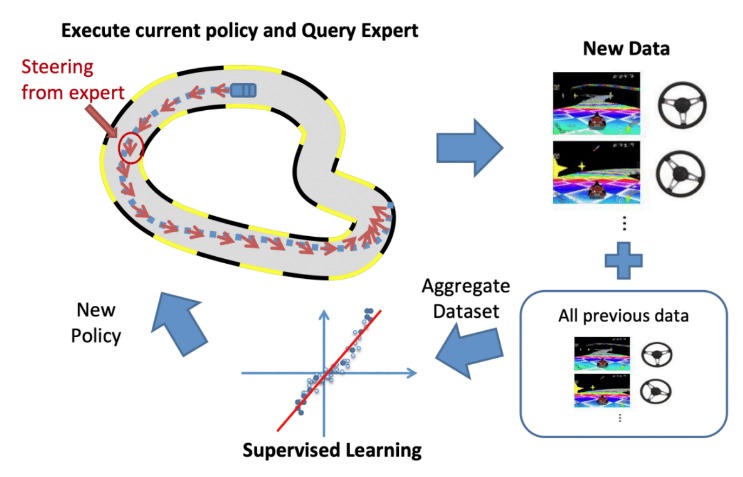
\includegraphics[width=0.8\textwidth]{dagger.png}
\caption{DAgger illustration}
\label{fig:dagger}
\end{figure}

The algorithm is presented in Algo 2.
\begin{algorithm}[H]
\caption{DAgger $\left(\beta, \pi^{*}, \Pi, \mathcal{E}\right)$}
\begin{algorithmic}[1]
\FOR{$k=1,\;\cdots,\;K$}
\STATE $\pi_{k}=\beta \pi^{*}+(1-\beta) \hat{\pi}_{k}$ \hfill $\triangleright$ mixture expert policy and hindsight optimal policy
\STATE  $\left\{s^{(t)}, a^{(t)}\right\}_{t=1}^{T} \sim \mathcal{E} \mid \pi_{k} $ \hfill$\triangleright$ off-policy trajectory sample
\STATE  $\mathcal{D} \leftarrow \mathcal{D} \cup\left\{s^{\left(t_{k}\right)}\right\}$ \hfill $\triangleright$ data aggregation
\STATE  $\hat{\pi}_{k+1}=\arg \min _{\pi \in \Pi} \sum_{d=1}^{|\mathcal{D}|} f\left(\pi\left(s^{(d)}\right), \pi^{*}\left(s^{(d)}\right)\right)$ \hfill $\triangleright$ hindsight optimal (leader) policy
\ENDFOR
\STATE \textbf{return} $\hat{\pi}$
\label{algo:dagger}
\end{algorithmic}
\end{algorithm}

Recall that online convex optimization is a generalization of online learning when the loss function is convex. We learn Follow-the-Leader algorithm as a general framework for online learning. If we can construct a convex loss function of the expert policy and the learner  policy, Interactive Imitation Learning is
Online Convex Optimization and DAgger is just Follow-the-Leader algorithm with the no-regret guarantee.

Here we summarize the pros and cons of DAgger as follows.\\
Pros:
\begin{itemize}
    \item Trajectory sampling implicitly accounts for sequential dependence of actions (addresses domain shift problem)
    \item Reduction of IL to online learning results in no-regret bounds
\end{itemize}
Cons:
\begin{itemize}
    \item Solving for the optimal policy for each iteration can be a costly optimization
    \item All mistakes are treated equally. No explicit reasoning about sequential dependence (e.g., future payoff, value function or cost-to-go)
\end{itemize}

\subsection{AggreVaTe}
The main improvement of Aggregate Values to Imitate (AggreVaTe\cite{ross2014reinforcement}) compared with DAgger is it starts to take sequential dependence (e.g. future payoff) into consideration, by assigning more penalty to more fatal mistake. It leverages cost-to-go information.

The algorithm is presented in Algo~3.
\begin{algorithm}[H]
\caption{AGGREVATE $\left(\beta, \pi^{*}, \Pi, \mathcal{E}\right)$}
\begin{algorithmic}[1]
\FOR{$k=1,\;\cdots,\;K$}
\STATE $\pi_{k}=\beta \pi^{*}+(1-\beta) \hat{\pi}_{k}$ \hfill $\triangleright$ mixture expert policy and optimal policy
\STATE  $t_{k} \sim[T] $ \hfill$\triangleright$ sample switch point
\STATE  $\left\{s^{(i)}\right\}_{i=0}^{t_{k}} \sim \mathcal{E} \mid \pi_{k}$ \hfill $\triangleright$ roll out with expert
\STATE   RECEIVE $\boldsymbol{Q}\left(s^{\left(t_{k}\right)}\right)$ \hfill $\triangleright$ roll out and get the Q value
\STATE  $\mathcal{D} \leftarrow \mathcal{D} \cup\left\{s^{\left(t_{k}\right)}, \boldsymbol{Q}\left(s^{\left(t_{k}\right)}\right)\right\}$ \hfill $\triangleright$ record roll out Q for each action
\STATE  $\hat{\pi}_{k+1}=\arg \min _{\pi} \sum_{d=1}^{|\mathcal{D}|} \sum_{a} \pi\left(a \mid s_{d}\right) Q^{*}\left(s_{d}, a\right)$ \hfill $\triangleright$ pick cost sensitive policy
\ENDFOR
\STATE \textbf{return} $\hat{\pi}$
\label{algo:aggrevate}
\end{algorithmic}
\end{algorithm}
AggreVaTe will stop at a random time step $t$ and start to take exploratory action, then follow the expert policy until we reach the end and get the Q value. Its cost sensitive policy will learn to minimize the probability of taking the action leading to low Q value by line 7. Notice that Q can be empirically calculated from Monte Carlo or TD($\lambda$) prediction.

In conclusion, the AggreVaTe will try to minize the \textbf{cost} of mistakes (vs. \textbf{number} of mistakes for DAgger), by asking expert the \textbf{consequence} of mistakes (vs. \textbf{occurence} of a mistake for DAgger).


\subsection{Comparisons}
In this section we will use Figure~\ref{fig:comp} and Table~\ref{tab:comp} to illustrate the major differences among Interactive IL, Passive IL, Active IL, Inverse Reinforcement Learning (IRL) and traditional Reinforcement Learning (RL). 

\begin{figure}[H]
\centering
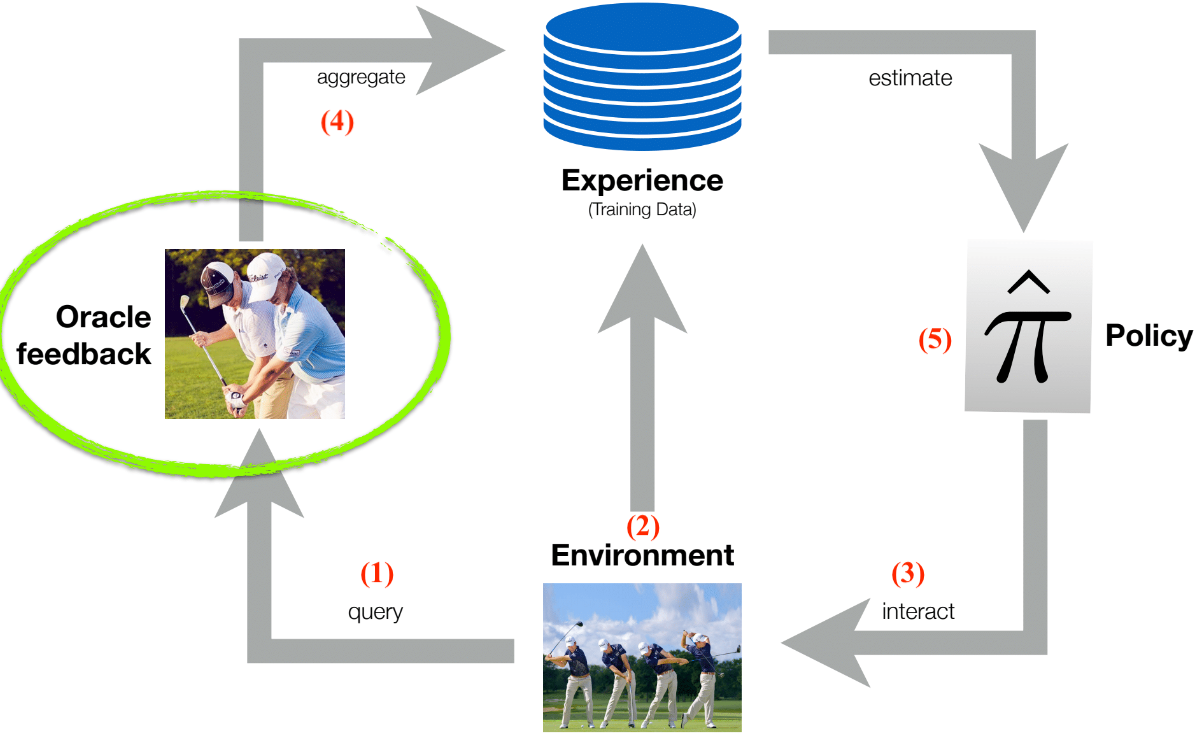
\includegraphics[width=0.8\textwidth]{comparison.png}
\caption{Graph used for comparison}
\label{fig:comp}
\end{figure}

\begin{table}[H]
\centering
\begin{tabular}{|c|c|c|c|c|c|}
\hline & Passive IL & Active IL & Interactive IL & Inverse RL & RL \\
\hline (1)  & no & no & yes & no & no\\
\hline (2)  & no & yes & yes & yes & yes\\
\hline (3)  & no & yes & yes & yes & yes \\
\hline (4)  & yes & yes & yes & yes & no\\
\hline (5)  & only policy $\hat{\mathbf{\pi}}$ & only policy $\hat{\mathbf{\pi}}$ & only policy $\hat{\mathbf{\pi}}$ & policy $\hat{\mathbf{\pi}}$ + reward $\hat{\mathbf{R}}$&only policy $\hat{\mathbf{\pi}}$\\
\hline
\end{tabular}
\caption{Difference among 5 algorithms. \textit{yes} means the algorithm have access.}
\label{tab:comp}
\end{table}


\subsection{Conclusion}
When it comes to sequential process which requires sequential decisions, things will become much more complicated. But with online learning and no-regret analyses, we can introduce different Imitation Learning algorithms to solve this difficult problem. Due to the design of Imitation Learning, we can avoid global explorations, which is much more efficient or even realizable when state/action space are infinite. Combining Imitation and Reinforcement can also train an agent outperforming our experts.


\newpage

% \section{Appendix}
% \subsection{More on IL} 



%\section*{References}
%Include your references here. Please cite any resources you found useful.	
%Populate the refs.bib file or list your references manually. Be consistent in formatting!
{
\bibliography{refs}
\bibliographystyle{abbrv}
}

%\section{Appendix}
%This section provides any relevant background material that was not covered in the lectures, but was found to be useful for understanding the material. 
%For example, derivations, theory underlying techniques employed, etc. 

%Additionally, this section can summarizes applications or extensions of these techniques found in the literature. 

\end{document} % Done!


